%% Author: Daniel Kaplan
%% Subject: Interpreting boxplots





Here is a boxplot:


\centerline{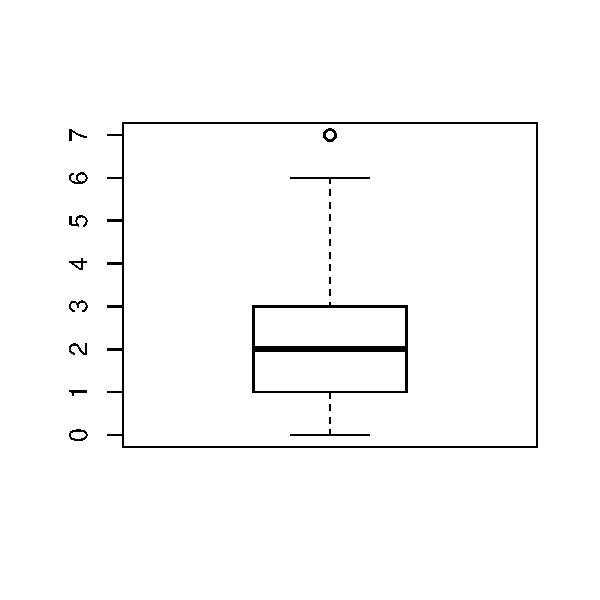
\includegraphics[width=2.5in]{Figures/AC128-plot1.pdf}}
\bigskip

Reading from the graph, answer the following:

\begin{enumerate}[(a)]
\item What is the median?

\SelectSetHoriz{2}{0,1,2,3,6,{Can't estimate from this graph}} 

\begin{AnswerText}
The boxplot displays the 25th, 50th, and 75th percentiles as the
bottom, middle, and top of the box.  
the 
\end{AnswerText}

\item What is the 75th percentile?

\SelectSetHoriz{3}{0,1,2,3,6,{Can't estimate from this graph}} 

\item What is the IQR?

\SelectSetHoriz{2}{0,1,2,3,4,6,{Can't estimate from this graph}} 

\begin{AnswerText}
The IQR is the distance between the 25th and 75th percentiles.
\end{AnswerText}

\item What is the 40th percentile?
\begin{MultipleChoice}
\wrong{between 0 and 1}
\correct{between 1 and 2}
\wrong{between 2 and 3}
\wrong{between 3 and 4}
\wrong{between 4 and 6}
\wrong{Can't estimate from this graph.}
\end{MultipleChoice}

\begin{AnswerText}
The 40th percentile {\bf must} be somewhere between the 25th and 50th
percentiles, both of which can be read off the graph.
\end{AnswerText}


\end{enumerate}

